\documentclass[fleqn]{article}
\usepackage{listingsutf8}
\lstset{basicstyle=\ttfamily, language=Octave} 
\usepackage[pdftex]{graphicx}
\usepackage[english]{babel} 
\usepackage[T1]{fontenc}
\usepackage[utf8]{inputenc}
\usepackage[parfill]{parskip}
\usepackage{tcolorbox}
\usepackage{verbatim}
\usepackage{listings}
\usepackage{xcolor}
\usepackage[export]{adjustbox}
\usepackage[fleqn]{amsmath}
\usepackage[font=small,labelfont=bf]{caption}
\usepackage{subfig}
\captionsetup{format=hang}
\captionsetup{justification=raggedright,singlelinecheck=false}

\lstset{
  basicstyle=\ttfamily,
  escapeinside=||
}

\renewcommand{\baselinestretch}{1.5}
\begin{document}

\begin{titlepage} % Suppresses displaying the page number on the title page and the subsequent page counts as page 1
	\newcommand{\HRule}{\rule{\linewidth}{0.5mm}} % Defines a new command for horizontal lines, change thickness here
	
	\center % Centre everything on the page
	
	%------------------------------------------------
	%	Headings
	%------------------------------------------------
	
	\textsc{\LARGE Fakulteta za računalništvo in informatiko, Univerza v Ljubljani}\\[1.5cm] % Main heading such as the name of your university/college
	
	\textsc{\Large Mathematical Modeling}\\[0.5cm] % Major heading such as course name
	
	\textsc{\large Third Home Assignment}\\[0.5cm] % Minor heading such as course title
	
	%------------------------------------------------
	%	Title
	%------------------------------------------------
	
	\HRule\\[0.4cm]
	
	{\huge\bfseries Report}\\[0.4cm] % Title of your document
	
	\HRule\\[1.5cm]
	
	%------------------------------------------------
	%	Author(s)
	%------------------------------------------------
	
	\begin{minipage}{0.4\textwidth}
		\begin{flushleft}
			\large
			\textit{Author}\\
			Jernej Vivod % Your name
		\end{flushleft}
	\end{minipage}
	~
	\begin{minipage}{0.4\textwidth}
		\begin{flushright}
			\large
			\textit{Lecturer}\\
			Dr. Neža Mramor Kosta
		\end{flushright}
	\end{minipage}
	
	% If you don't want a supervisor, uncomment the two lines below and comment the code above
	%{\large\textit{Author}}\\
	%John \textsc{Smith} % Your name
	
	%------------------------------------------------
	%	Date
	%------------------------------------------------
	
	\vfill\vfill\vfill % Position the date 3/4 down the remaining page
	
	{\large\today} % Date, change the \today to a set date if you want to be precise
	
	%------------------------------------------------
	%	Logo
	%------------------------------------------------
	
	%\vfill\vfill
	%\includegraphics[width=0.2\textwidth]{placeholder.jpg}\\[1cm] % Include a department/university logo - this will require the graphicx package
	 
	%----------------------------------------------------------------------------------------
	
	\vfill % Push the date up 1/4 of the remaining page
	
\end{titlepage}
\tableofcontents
\newpage


\section{Problem Statement}

We are given a Matrix V that represents the values of a function $f(i, j) = V_{ij}$ for integer arguments $(i, j)$.

Our goal is to interpolate the data with some function or a set of functions to produce a smooth surface.

The task should be solved on the domain $[1, n] \times [1, m]$ by individually interpolating the squares of unit size, making sure the function is continuous with the function of the neighboring unit square and pasting together the functions.

This solution is based on the concept of the so called partition of unity.

\subsection{MATLAB/Octave Implementation Goals}

We are tasked with implementing two MATLAB/Octave functions relating to this problem.

The first function is given by the header

\begin{tcolorbox}
\begin{verbatim}
Z = interpolationFunction(data, len);
\end{verbatim}.
\end{tcolorbox}

This function computes the values of the unit square interpolating function on a $len \times len$ grid of equally spaced points from the domain $[0,1] \times [0,1]$.

The data required for the unit square computations is stored in the data variable.

The second function is given by the header

\begin{tcolorbox}
\begin{verbatim}
interpolation(V, len)
\end{verbatim}.
\end{tcolorbox}

This function should first plot the data contained in the V matrix and the evaluations of the interpolating function. The interpolating function should be evaluated at each unit square comprising the matrix in the same fashion as in the interpolationFunction function. These results should them be concatenated to from a matrix representing evaluations of the concatenated interpolating functions of matrix V. The function should then also plot this concatenated matrix alongside the first plot. Both plots should be done using the surf or mesh functions.

\section{Interpolating the Unit Square}

This subsection describes the computation of the interpolating function on the unit square $K = [0, 1] \times [0, 1]$.

Let us assume we are given the values of the function on the vertices of the unit square $A(0,0), \ B(1, 0), \ C(0, 1) \ , D(1, 1)$. Let us denote these values by $a, \ b, \ ,c, \ d$. Assuma that we are also given the values of the partial derivatives in the x and y directions for the function in the vertices of the unit square $K$. Denote these values by $a_{x}, \ b_{x}, \ c_{x}, \ d_{x}$ and $a_{y}, \ b_{y}, \ c_{y}, \ d_{y}$ respectively.

The next step is to compute the weighting functions that will give weight to each vertex value contribution depending on where the interpolating function is evaluated.

This weighting function associated with each vertex should be equal to 1 in that vertex and 0 in every other vertex. We also want this function to be continuous.

Let us define a function that will help construct the weighting functions. We are looking for a 3. order polynomial with that satisfies the conditions 

$p(0)=1, \ p(1) = 0, \ p'(0)=0, \ p'(1) = 0$. 

Here, we are in fact interpolating the values $(0, 1)$ and $(1, 0)$ using the cubic interpolation method. Since we do not know the derivative of the function, we can simply use 0 as the derivative value at each interpolation point.

First, we write the general equation for a 3. order polynomial
\begin{equation}
p(x) = ax^3 + bx^2 + cx + d
\end{equation}

The derivative of this polynomial with respect to x is
\begin{equation}
p'(x) = 3ax^2 + 2bx + c
\end{equation}

Evaluating this general equation and its derivative at the known points yields us a system of 4 equations with 4 unknowns:
\begin{align}
\begin{split}
& p(0) = d = 1 \\
& p(1) = a + b + c + d = 0 \\
& p'(0) = c = 0 \\
& p'(1) = 3a + 2b + c = 0 \\
\end{split}
\end{align}

This can be written compactly with the following system of linear equations in matrix form as
\begin{equation}
\begin{bmatrix} 0 & 0 & 0 & 1 \\ 1 & 1 & 1 & 1 \\ 0 & 0 & 1 & 0 \\ 3 & 2 & 1 & 0 \end{bmatrix} \begin{bmatrix} a \\ b \\ c \\ d \end{bmatrix} = \begin{bmatrix} 1 \\ 0 \\ 0 \\ 0 \end{bmatrix}
\end{equation}

which can then be solved for the vector of coefficients b.

\newpage

This can be easily achieved in MATLAB/Octave to give us the vector of coefficients for the desired polynomial.

\begin{tcolorbox}
	\begin{verbatim}
>> A = [0 0 0 1;
     1 1 1 1; 
     0 0 1 0; 
     3 2 1 0];        
>> b = [1; 0; 0; 0];
>> coeff = A\b
coeff =

   2.00000
  -3.00000
   0.00000
   1.00000
	\end{verbatim}
\end{tcolorbox}

The polynomial that satisfies our conditions is therefore 
\begin{equation}
p(x) = 2x^3 - 3x^2 + 1
\end{equation}

We can use this polynomial to construct the weighting functions with the desired properties described above:
\begin{align}
\begin{split}
& w_{A}(x, y) = p(x)p(y) \\
& w_{B}(x, y) = (1 - p(x))p(y) \\
& w_{C}(x, y) = p(x)(1 - p(y)) \\
& w_{D}(x, y) = (1 - p(x))(1 - p(y))
\end{split}
\end{align}

Let us also define auxiliary functions that describe the change of each vertex value with respect to position in the unit square. We define these functions by taking into account the value of the interpolating function in a specific vertex and the derivatives of the function in different directions.
\begin{align}
\begin{split}
& f_{a}(x, y) = a + a_{x}x + a_{y}y \\
& f_{b}(x, y) = b + b_{x}(x - 1) + b_{y}y \\
& f_{c}(x, y) = c + c_{x}x + c_{y}(y - 1) \\
& f_{d}(x, y) = d + d_{x}(x - 1) + d_{y}(y - 1)
\end{split}
\end{align}

We now have all the information needed to define the interpolating function $f$ that interpolates the values in the vertices of the unit square $K$:
\begin{equation}
f = f_{A}w_{A} + f_{B}w_{B} + f_{C}w_{c} + f_{d}w_{d}
\end{equation}

where the argument is omitted for brevity.

\section{Some Properties of the Constructed Unit Square}

In this section we would like to show some important properties that hold for our method of treatment of an arbitrary unit square $K$.

\subsection{Showing that the Weights Sum to 1}

In this subsection we will show that the sum of the weighting functions is always equal to 1 irrespective of the values of $x$ and $y$.

Let us first write the sum of the weighting functions in terms of their definitions
\begin{align*}
w_{a} + w_{b} + w_{c} + w_{d} = p(x)p(y) + (1 - p(x))p(y) + p(x)(1 - p(y)) + (1 - p(x))(1 - p(y))
\end{align*}
Getting rid of the parenthesis yields us
\begin{align*}
\sum w = p(x)p(y) + p(y) - p(x)p(y) + p(x) - p(x)p(y) + 1 - p(y) - p(x) + p(x)p(y))
\end{align*}
where all terms but the constant 1 cancel out and we are left with the following expression.
\begin{align*}
\sum w = 1
\end{align*}

We have shown that the sum of the weighting functions is always equal to 1 and does not depend on the values of the functions themselves nor on the coordinates $(x, y)$.

\subsection{Showing that the Values of the Interpolating Function and its Partial Derivatives at a Given Vertex Depend only on the Data that Refers to that Particular Unit Square Vertex}

Consider the unit square vertex $a$ with coordinates $(0, 0)$. We would like to show that the interpolating function and its derivatives depend only on the data referring to that that vertex (i.e. $a, \ a_{x}, \ a_{y}$). Let us first consider the weighting function associated with vertex a. This weighting function is written as $w_{A}(x, y) = p(x)p(y)$. Since the vertex $a$ has coordinates $(0, 0)$ within the unit square, the weighting function is evaluated at the vertex as $w_{A}(x, y) = p(0)p(0) = 2 \cdot 0^3 - 3 \cdot 0^2 + 1 =  1$.

But what about the weighting functions associated with the other three vertices $b$, $c$ and $d$? Let us perform the same computation for their coordinates within the unit square.

Recall that the desired property of the polynomial $p(x)$ is that $p(0) = 1$ and $p(1) = 0$.
\begin{align}
\begin{split}
& w_{a}(0, 0) = p(0)p(0) = 1 \cdot 1 = 1 \\
& w_{b}(0, 0) = (1 - p(0))p(0) = 0 \cdot 1 = 0 \\
& w_{c}(0, 0) = p(0)(1 - p(0)) = 1 \cdot 0 = 0 \\
& w_{d}(0, 0) = (1 - p(0))(1 - p(0)) = 0
\end{split}
\end{align}

Now let us recall the interpolation formula

$f = f_{A}w_{A} + f_{B}w_{B} + f_{C}w_{c} + f_{d}w_{d}$.

Using the compute values for the weighting function, the equation for the vertex a then simply becomes

$f = f_{A}$

Recall that the auxiliary function $f_{A}$ is defined as 
$f_{A}(x, y) = a + a_{x}x + a_{y}y$.

Since the unit square coordinates of the vertex $a$ are $(0, 0)$ the equation becomes

$f_{A}(0, 0) = a + a_{x}0 + a_{y}0 = a$.

We can clearly see that the evaluation of the interpolating function at the vertex $a$ is precisely equal to the value $a$. This shows that the interpolating function will go precisely through the initial interpolation points.

Similar computations can be carried out for the other three vertices to show that the same holds for vertices $b$, $c$ and $d$ as well.

\subsection{Showing that the Values of the Interpolating Function and its Partial Derivatives at a Given Unit Square Edge Depend only on the Data that Refers to that Particular Edge}

Consider the domain on te unit square given by $[0, 0] \times [0, 1]$. This domain represents all points that lie on the left edge of the unit square given in cartesian coordinates. Notice that the x coordinate of all the points is equal to $0$ everywhere on the domain.

\pagebreak
Let $k \in [0, 1]$. The weighting functions can then be written as:

\begin{align}
\begin{split}
& w_{a}(0, k) = p(0)p(k) = p(k)\\
& w_{b}(0, k) = (1 - p(0))p(k) = 0 \cdot p(k) = 0 \\
& w_{c}(0, k) = p(0)(1 - p(k)) = 1 - p(k) \\
& w_{d}(0, k) = (1 - p(0))(1 - p(k)) = 0 \cdot (1 - p(k)) = 0
\end{split}
\end{align}

The interpolating function $f$ therefore reduces to

$f = f_{A} \cdot p(k) + f_{C} \cdot (1 - p(k))$.

We know that the computation of the auxiliary function associated with a particular vertex depend only on the values associated with that vertex. In this case

$f_{A}(x, y) = a + a_{x}x + a_{y}y$ and $f_{c}(x, y) = c + c_{x}x + c_{y}(y - 1)$

where vertices $A$ and $C$ both lie on the edge we have chosen at the start. We can show that this same property holds for all the other vertices.

\subsection{Computing the Values of the Interpolating Function and its Partial Derivatives at the Vertices of the Unit Square}

Recall the formula for the interpolating function of the given unit square $K$.

$f = f_{A}w_{A} + f_{B}w_{B} + f_{C}w_{c} + f_{d}w_{d}$

Above we have shown that at a specific vertex $v \in {a, \ b, \ c, \ d}$ the interpolating function reduces to $f = f_{v}$, where $v \in {a, \ b, \ c, \ d}$.

The auxiliary function $f_{v}$, $v \in {a, \ b, \ c, \ d}$ is defined as

\begin{align*}
f_{v} = 
\begin{cases} 
      a + a_{x}x + a_{y}y & v := a \\
      b + b_{x}(x - 1) + b_{y}y & v := b \\
      c + c_{x}x + c_{y}(y - 1) & v := c \\
      d + d_{x}(x - 1) + d_{y}(y - 1) & v := d
\end{cases}
\end{align*}

Let us show how this function behaves at a specific vertex. Take the vertex denoted by $a$ with coordinates $(0, 0)$ as a basic example.

Notice the for vertex $a$, $x, y = 0$. So the equation further reduces to

$f_{a}(0, 0) = a$

Where a is a constant value - an interpolation point given in the initial data.

This, of course, means that

$\frac{\partial f_{a}}{x} = \frac{\partial f_{a}}{y} = 0$. 

We can easily show the same holds for the other vertices $b$, $c$ and $d$.

\section{MATLAB/Octave Implementations}

\subsection{MATLAB/Octave Implementation - interpolationFunction}

This subsection describes the implementation of the MATLAB/Octave function described by the header

\begin{tcolorbox}
\begin{verbatim}
Z = interpolationFunction(data, len)
\end{verbatim}
\end{tcolorbox}

This function evaluates the interpolating function constructed from interpolating the vertices of a unit square described by the data argument on a grid of dimensions $len \times len$ consisting of equally spaced points from $[0, 1] \times [0, 1]$. The result is returned in matrix form.

The implementation described here implements the data variable as a $4 \times 3$ matrix where each row contains data for a different vertex (in alphabetical order)
\begin{align*}
data = \begin{bmatrix} a & a_{x} & a_{y} \\ b & b_{x} & b_{y} \\ c & c_{x} & c_{y} \\ d & d_{x} & d_{y} \end{bmatrix}
\end{align*}

The grid of points at which we would like to evaluate the interpolating function can be written using the linspace and meshgrid functions. In this specific implementation we will combine the results of the meshgrid function into a 3 dimensional matrix where each cell contains both the value of $x$ and $y$. This can be achieved using the cat function.

\begin{tcolorbox}
\begin{verbatim}
% Create grid of x and y values on interval [0, 1] 
% with dimensions len x len.
x_pts = linspace(0, 1, len);
y_pts = linspace(0, 1, len);
[X, Y] = meshgrid(x_pts, y_pts);
  
% Create a three dimensional matrix for easier 
% visualization of the grid.
% Each cell contains its x and y value.
xy_grid = cat(3, X, Y);
\end{verbatim}
\end{tcolorbox}

The next step is to write the interpolating function through the values at the vertices at the unit square. 

Let us first extract the values from the data matrix described above.

\begin{tcolorbox}
\begin{verbatim}
% Extract values from the data matrix.
a = data(1, 1);
dx_a = data(1, 2);
dy_a = data(1, 3);
b = data(2, 1);
dx_b = data(2, 2);
dy_b = data(2, 3);
c = data(3, 1);
dx_c = data(3, 2);
dy_c = data(3, 3);
d = data(4, 1);
dx_d = data(4, 2);
dy_d = data(4, 3);
\end{verbatim}
\end{tcolorbox}

Now we compute the third degree polynomial discussed in the previous section.

\begin{tcolorbox}
\begin{verbatim}
% Compute third degree polynomial p(x) with properties
% p(0) = 1, p'(0) = 0, p(1) = 0, p'(1) = 0.
%
% Polynomial can be written as p(x) = ax^3 + bx^2 + cx + d.
% It's derivative with respect to x is 3ax^2 + 2bx + c.
% 
% Pass required x values and set equal to result.
% Solve resulting system of linear equations

A = [0 0 0 1; 1 1 1 1; 0 0 1 0; 3 2 1 0];
sol = [1; 0; 0; 0];
coeff = A\sol;

\end{verbatim}
\end{tcolorbox}

This gives us enough data to define the weighting functions

\begin{small}
\begin{tcolorbox}
\begin{verbatim}
% The properties of this polynomial guarantee that the 
% derivative values on the edges of the unit squares 
% will match (will be zero)

% Compute weights.
weight_A = @(x, y) polyval(coeff, x)*polyval(coeff, y);
weight_B = @(x, y) (1 - polyval(coeff, x))*polyval(coeff, y);
weight_C = @(x, y) polyval(coeff, x)*(1 - polyval(coeff, y));
weight_D = @(x, y) (1 - polyval(coeff, x))*(1 - polyval(coeff, y));
\end{verbatim}
\end{tcolorbox}
\end{small}

And also the auxiliary functions discussed in the previous section.

\begin{tcolorbox}
\begin{verbatim}
% Compute auxilliary functions.
aux_A = @(x, y) a + dx_a.*x + dy_a.*y;
aux_B = @(x, y) b + dx_b.*(x - 1) + dy_b.*y;
aux_C = @(x, y) c + dx_c.*x + dy_c.*(y - 1);
aux_D = @(x, y) d + dx_d.*(x - 1) + dy_d.*(y - 1);
\end{verbatim}
\end{tcolorbox}

And finally, let us define the interpolating function,

\begin{tcolorbox}
\begin{verbatim}
% Compute interpolating function on the given unit square
i_func = @(x, y) aux_A(x, y) .* weight_A(x, y) +...
aux_B(x, y) .* weight_B(x, y) +...
aux_C(x, y) .* weight_C(x, y) +...
aux_D(x, y) .* weight_D(x, y);
\end{verbatim}
\end{tcolorbox}

This function can now be called for every pair of $x$ and $y$ values in the $len \times len$ grid discussed above. We return this value as we will also need it in the next function.

\subsection{MATLAB/Octave Implementation - interpolation}

This subsection describes the implementation of the MATLAB/Octave function described by the header

\begin{tcolorbox}
\begin{verbatim}
interpolation(V, len)
\end{verbatim}
\end{tcolorbox}

Computes and evaluates the interpolation of the data in matrix $V$ by individually
interpolating the values in unit squares and pasting together the results of evaluating each
unit square's interpolating function over equally spaced matrices of dimensions $len \times len$ with values from interval $[0, 1] \times [0, 1]$. The function plots both the initial data points and the results of interpolating function evaluations using the surf function.

The idea is to go over every unit square in the given matrix $V$ and compute the interpolating function and its evaluation (use the previous function) and then paste together the result into another matrix.

Here we show the computation of the data structure for a single unit square taken from the matrix V. This computation should be repeated for each unit square comprising the matrix V. 

The derivatives at points in a certain direction are set equal to the slope of the line passing through the neighboring points in that direction which can be easily computed using the familiar "rise over run" formula.
\begin{small}
\begin{tcolorbox}
\begin{verbatim}
unit_square = [V(i,j), V(i, j + 1); V(i + 1, j), V(i + 1, j + 1)];
      
% Construct data matrix.
% Compute function values and derivative values.
% The value of the derivative is the slope of 
% the line between the neighboring points
% in the derivative direction.

% See solution.pdf for more details.
a = V(i, j);
b = V(i, j + 1);
c = V(i + 1, j);
d = V(i + 1, j + 1);
dx_a = (V(i, j + 1) - V(i, j - 1))/2;
dy_a = (V(i + 1, j) - V(i - 1, j))/2;
dx_b = (V(i, j + 1 + 1) - V(i, j))/2;
dy_b = (V(i + 1, j + 1) - V(i - 1, j + 1))/2;
dx_c = (V(i + 1, j + 1) - V(i + 1, j - 1))/2;
dy_c = (V(i + 1 + 1, j) - V(i, j))/2;
dx_d = (V(i + 1, j + 2) - V(i + 1, j))/2;
dy_d = (V(i + 1 + 1, j + 1) - V(i, j + 1))/2;
      
% Create the data matrix for the unit square.
data = [a, dx_a, dy_a; b, dx_b, dy_b; c, dx_c, dy_c; d, dx_d, dy_d];
\end{verbatim}
\end{tcolorbox}
\end{small}

Finally, the function plots both the the original matrix V and the matrix of interpolating function evaluations side by side.

The results and plots of both the \textbf{\textit{interpolationFunction}} function and the \textbf{\textit{interpolation}} function are described in the next section.

\section{MATLAB/Octave Implementation - Results and Plots}

This section concisely describes the results of calling the implemented MATLAB/Octave functions with randomly generated data. All input matrices were generated by the \textbf{\textit{rand}} function. The \textit{len} variable is always set equal to 10.

\subsection{interpolationFunction}

function header
\begin{tcolorbox}
\begin{verbatim}
Z = interpolationFunction(data, len);
\end{verbatim}
\end{tcolorbox}

Values of the passed arguments

\begin{tcolorbox}
\begin{verbatim}
>> data
data =

   0.292964   0.098634   0.154782
   0.787147   0.219812   0.299968
   0.485641   0.286575   0.649834
   0.670497   0.231538   0.773773

>> len
len =  10
\end{verbatim}
\end{tcolorbox}


\begin{figure}[!ht]
    \centering
    \subfloat[Plotting the original data in the vertices of the given unit square as points in space]{{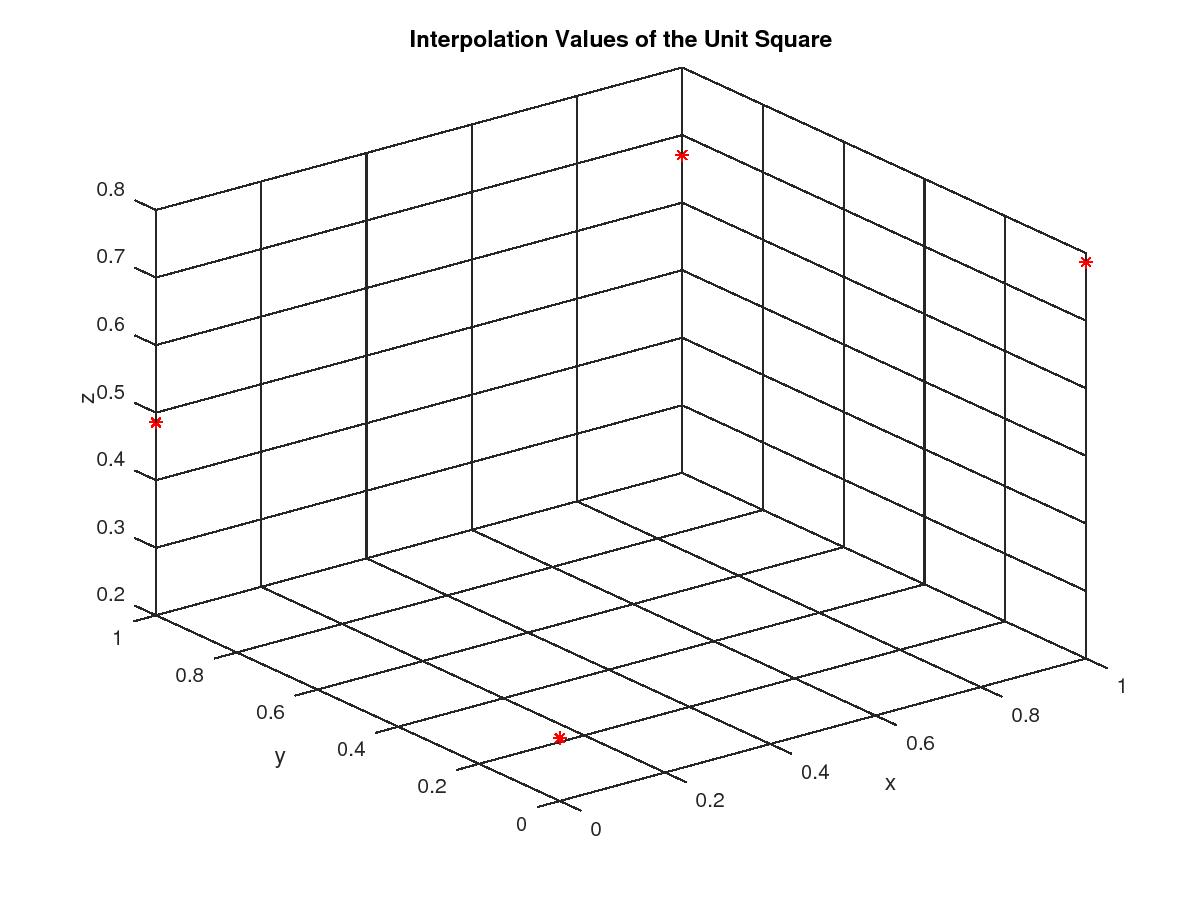
\includegraphics[width=5cm]{plot_usquare_points} }}%
    \qquad
    \subfloat[Plotting the resulting matrix Z as points in space]{{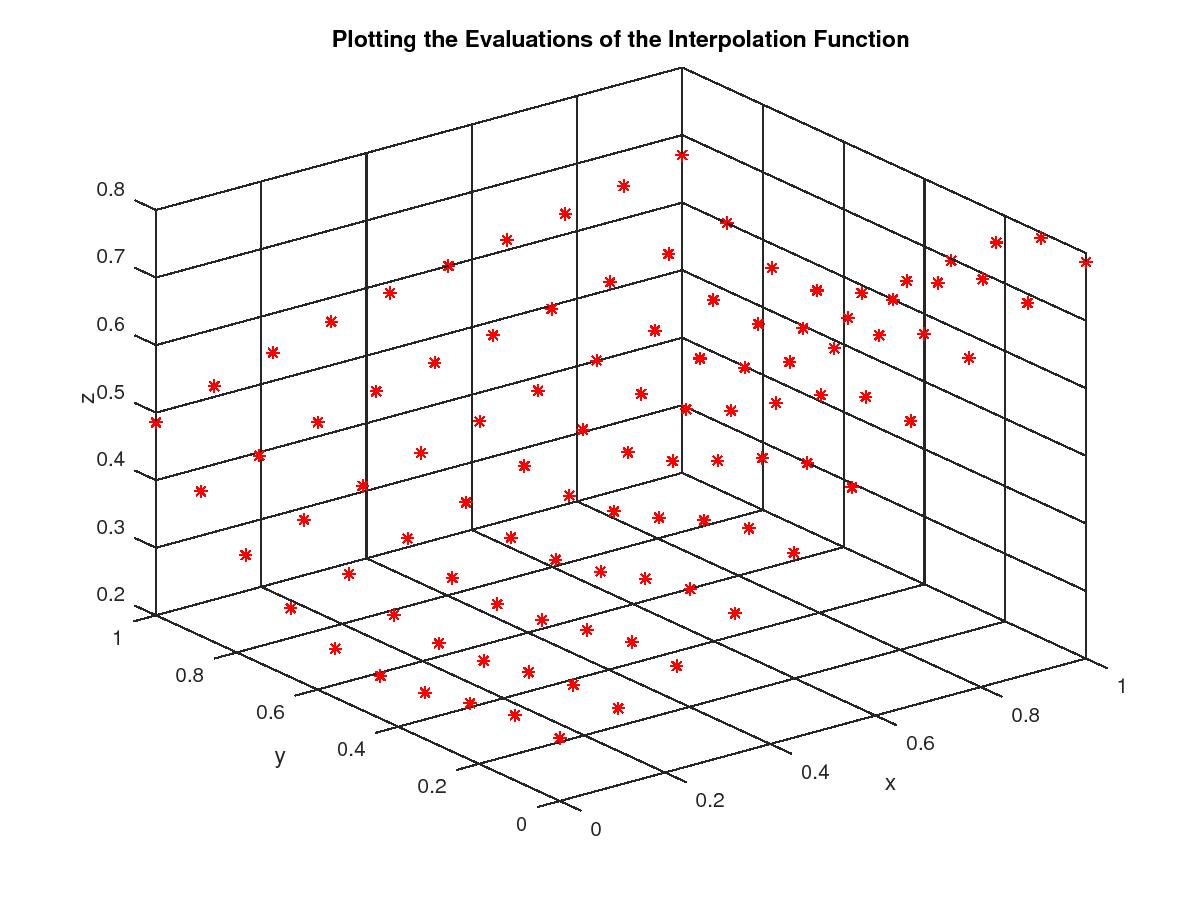
\includegraphics[width=5cm]{plot_usquare_points_interpolated} }}%
    \caption{Original points in the vertices and the evaluations of the interpolating function}%
    \label{fig:example}%
\end{figure}

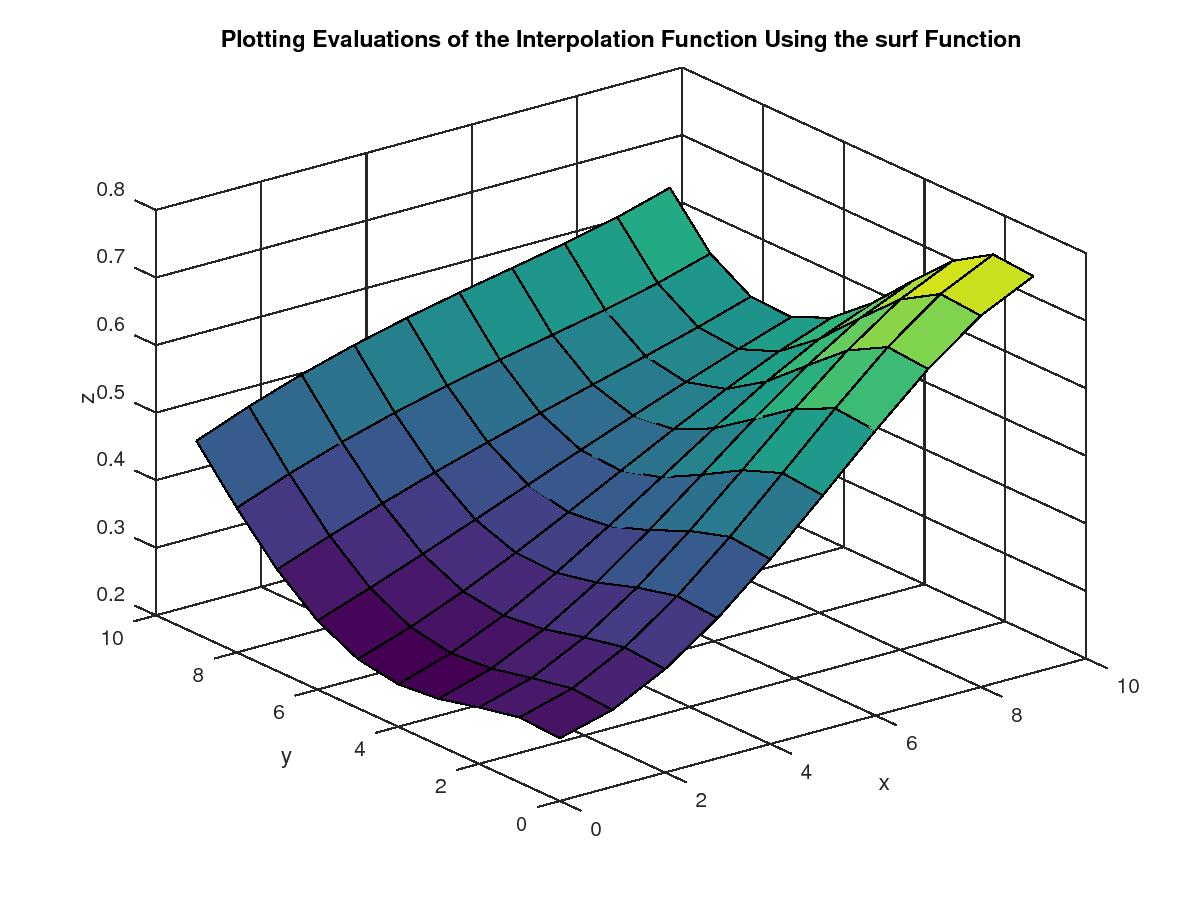
\includegraphics[scale=0.5, inner]{plot_usquare_points_interpolated_surf}
\captionof{figure}{Plotting the resulting matrix Z as a linearly interpolated surface using the surf function}

\newpage

\subsection{interpolation}

function header
\vspace{2mm}
\begin{small}
\begin{tcolorbox}
\begin{verbatim}
interpolation(V, len);
\end{verbatim}
\end{tcolorbox}
\end{small}

Values of the passed arguments
\vspace{2mm}
\begin{small}
\begin{tcolorbox}
\begin{verbatim}
>> V
V =

   0.249177   0.812302   0.822951   0.258785   0.403645
   0.494038   0.567649   0.958979   0.328572   0.499041
   0.220710   0.530066   0.678519   0.845553   0.309189
   0.022464   0.056340   0.258789   0.964440   0.265094
   0.933197   0.266604   0.022494   0.445106   0.202928

>> len
len =  10
\end{verbatim}
\end{tcolorbox}
\end{small}

\newpage

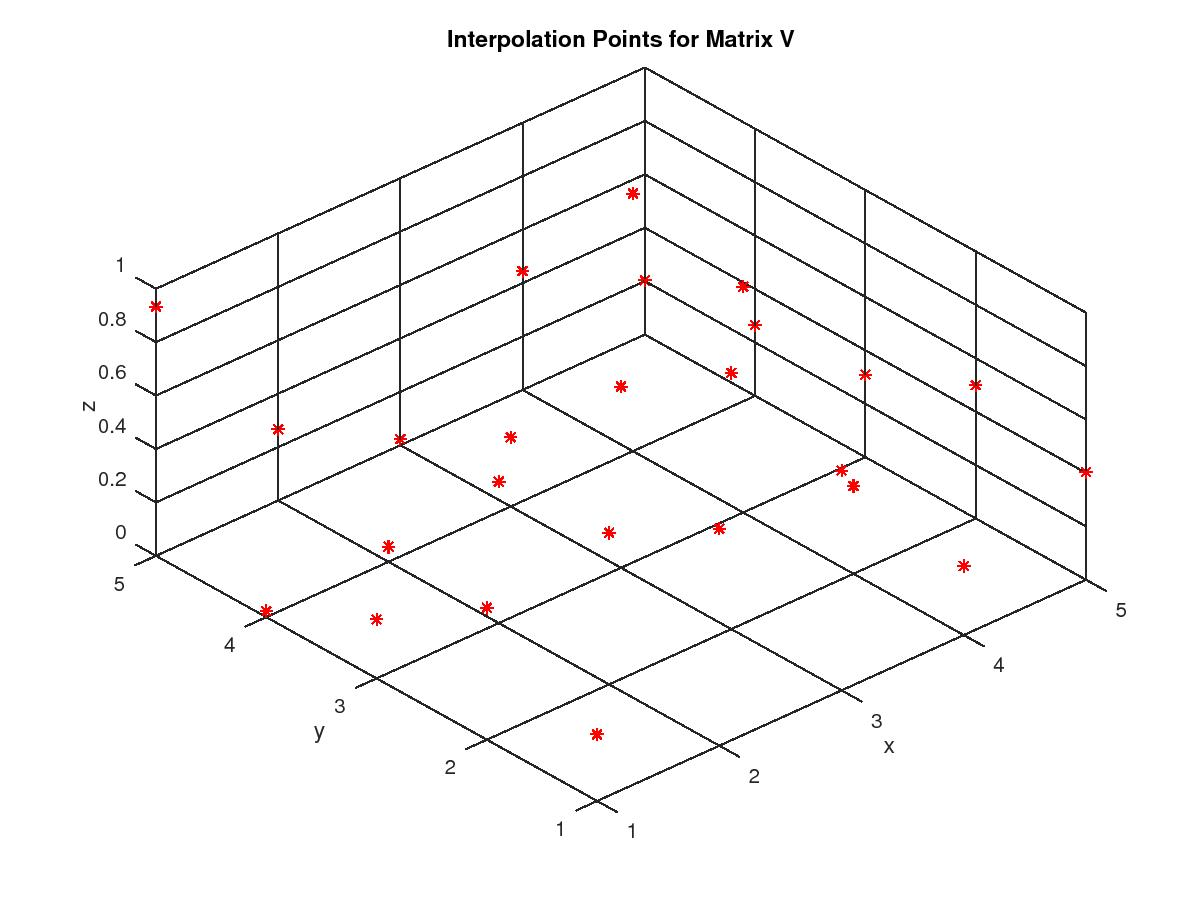
\includegraphics[scale=0.5, inner]{V_plot3}
\captionof{figure}{Plotting the data matrix V as points in space}

\vspace{10mm}

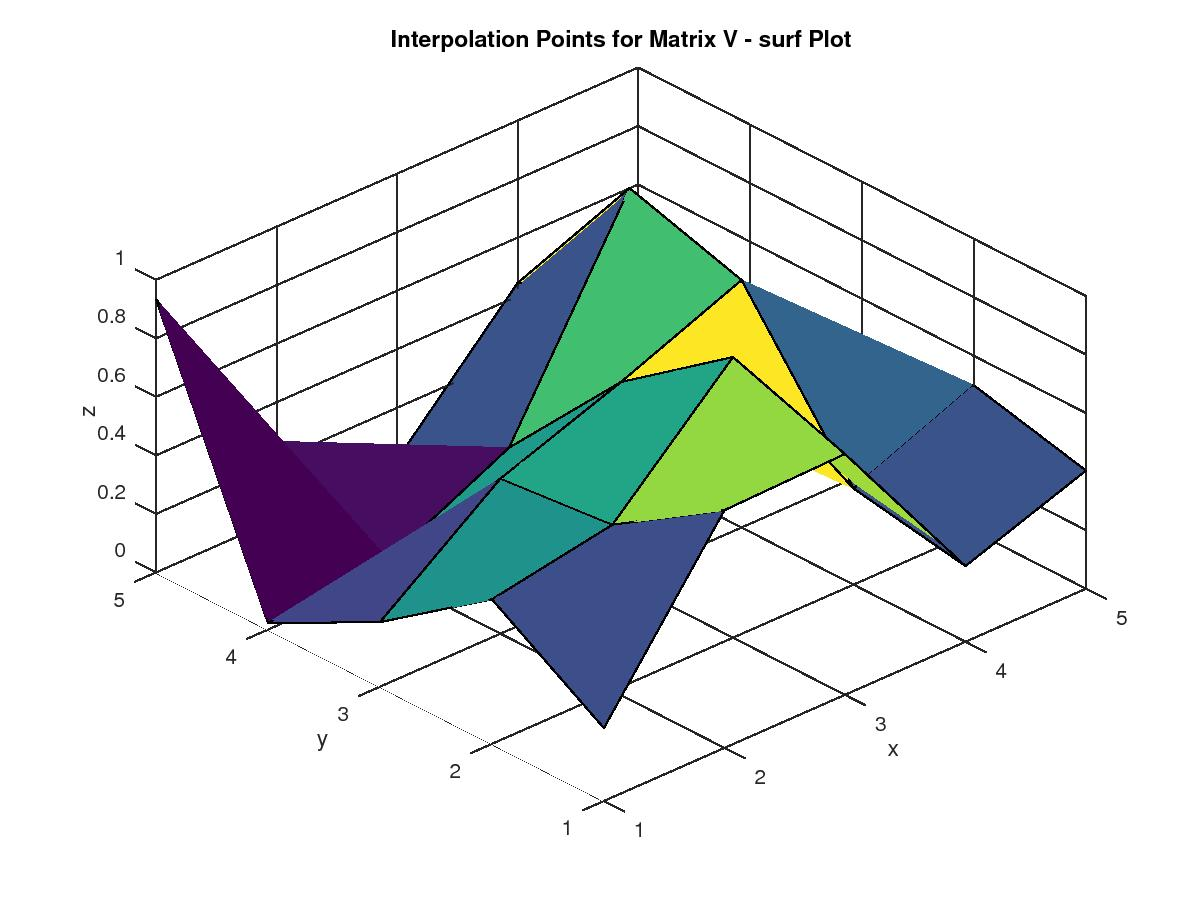
\includegraphics[scale=0.5, inner]{V_surf}
\captionof{figure}{Plotting the data matrix V as a linearly interpolated surface using the surf function}


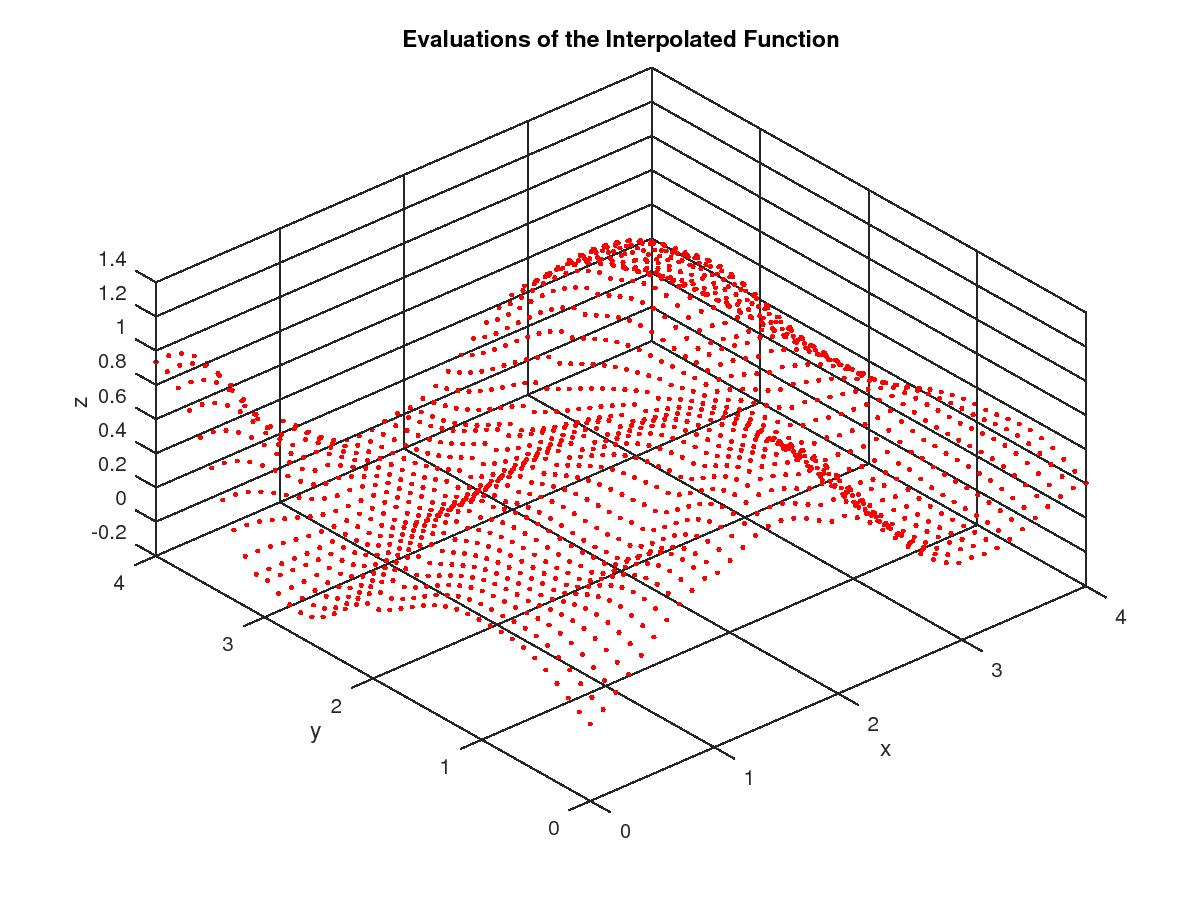
\includegraphics[scale=0.5, inner]{res_plot3}
\captionof{figure}{Plotting the result of the evaluation the interpolating function as points in space}

\vspace{10mm}

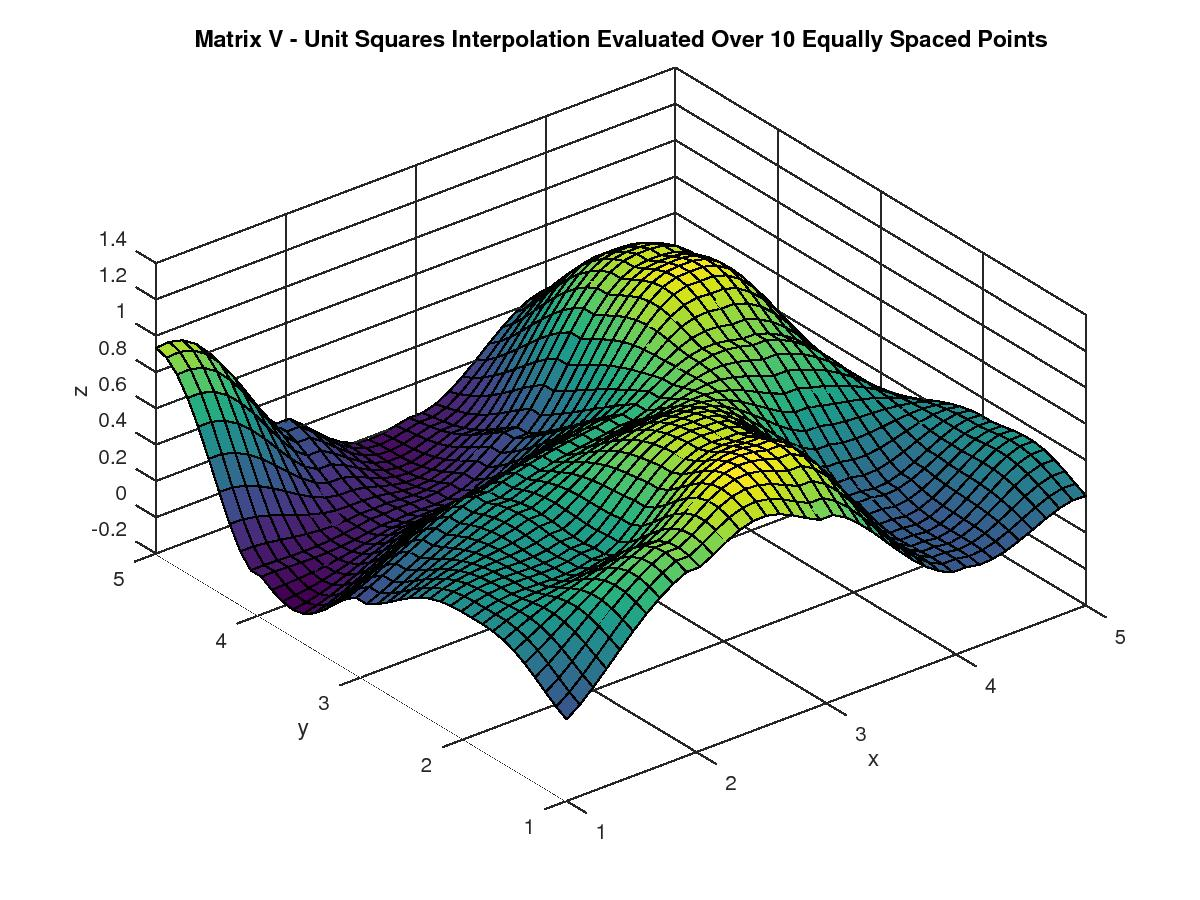
\includegraphics[scale=0.5, inner]{res_surf}
\captionof{figure}{Plotting the result of the evaluation the interpolating function as a linearly interpolated surface using the surf function
}

\end{document}